\clearpage

\subsection{Reticolo: determinazione del passo del reticolo}
Un fascio collimato di luce di lunghezza d'onda nota viene fatto passare attraverso un reticolo per poterne determinare il passo tramite la condizione di interferenza:
    $$ d\sin\theta = n\lambda $$
Vengono quindi effettuate misure dell'angolo a cui compaiono le varie righe spettrali (massimi di interferenza).
%
Se il reticolo è posizionato perpendicolarmente al fascio collimato emesso e noto che la riga gialla della lampada al sodio ha lunghezza d'onda $ \lambda = 589 $ [nm], si stima il passo del reticolo con la seguente relazione

\begin{equation}
d = \frac{ 589 n }{ \sin\theta }
\end{equation}
% Fit
%
%    \begin{figure}[H]
%    \centering
%    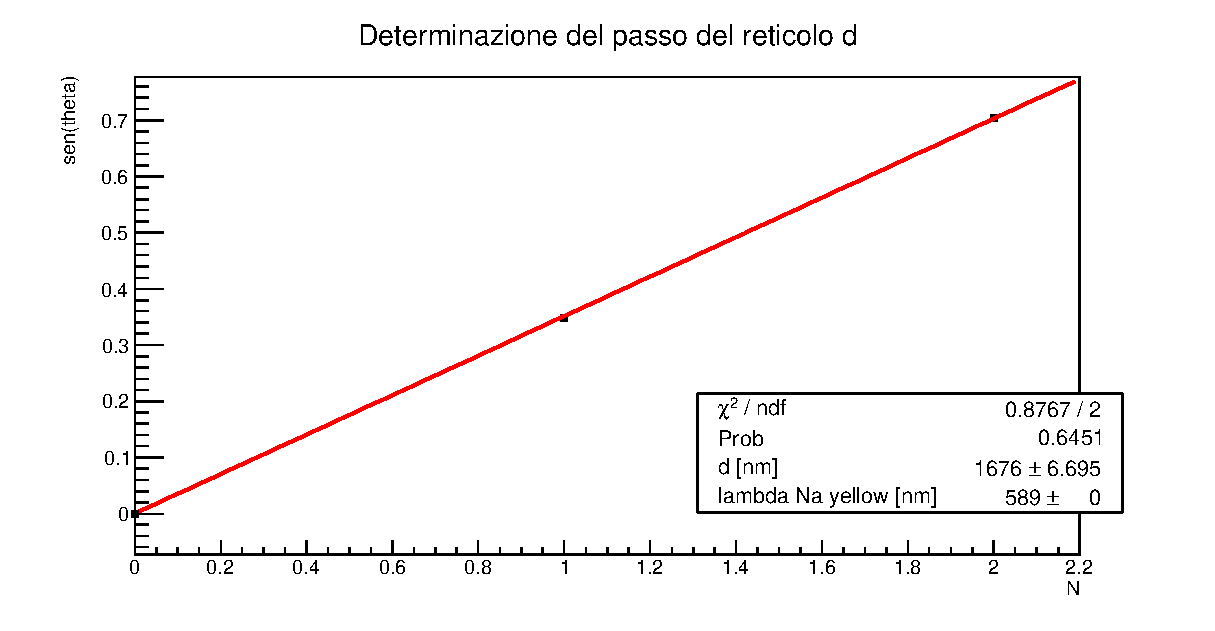
\includegraphics[scale=0.8]{Grafici/O3_P1_1_d.eps}
%    %\caption{}
%    \label{fig:C3_P2_RL}
%    \end{figure} 
%
%
%Fit usato: $ y = [1]/[0] x$\\
%dove $y = \sin(\theta)$ mediato (non corretto perchè non c'è bisogno, %sono simmetrici entro l'errore), $x = n$. Il parametro fissato è  $[1] = %\lambda_{yellow} = 589$ nm, e il parametro da stimare è $[0] = d$.\\\\
%
% Passo del reticolo stimato dal fit:
% $$d = 1676 \pm 7 \mathrm{ nm}$$
%
%
\begin{table}[H]
    \begin{center}
    \begin{tabular}{|l r|c|c|c|}
    \hline
            &   Ordine  &   $\theta$    & $\sin\theta$  &   d   \\
            &           &   rad         &   -           &   nm  \\
            &           &   $\pm0.01$   &   $\pm 0.004$ &   -   \\
        \hline
        sx  &   1       & 0.351         & 0.344         & 1713 \\ 
        dx  &   1       & 0.360         & 0.352         & 1671 \\ 
        \hline
        sx  &   2       & 0.748         & 0.680         & 1732 \\ 
        dx  &   2       & 0.797         & 0.715         & 1646 \\ 
        \hline
    \end{tabular}
    \end{center}
    \caption{ Posizioni angolari dei primi due massimi. Lampada al sodio. $\lambda = 589$ [nm] }
    \label{O3_P1_d}
\end{table}
%
%
Il valore di riferimento atteso è pari ad un passo di $1.667$ [nm] relativo a $600$ fenditure al [$\mu$m]. Questo dato possiede un errore intrinseco sul numero di linee. Non potendo stimare tale errore, assumiamo come valore teorico $1.67$ $\mu m$ consapevoli del fatto che possiede un errore.\\
Per calcolare l'errore di d è stata usata la formula di propagazione.
%
%
\begin{table}[H]
    \begin{center}
    \begin{tabular}{|l r|}
    \hline
        Valore stimato & $1.69 \pm 0.02$ $\mu m$ \\
        Valore di riferimento & $1.67$ $\mu m$ \\ 
    \hline
    \end{tabular}
    \end{center}
\end{table}
%
Considerati gli errori sperimentali, il valore trovato per $d$ è in buon accordo con quello teorico. Si esclude quindi l'eventuaità di asimmetria del sistema o di non perpendicolarità del fascio incidente